\documentclass{article}

\usepackage{graphicx,tikz}
\usepackage{fullpage}
\usepackage{amsthm}
\usepackage{amssymb}
\usepackage{amsmath}
\usepackage{algorithm}
\usepackage{algorithmicx}
\usepackage{algpseudocode}
\usepackage{booktabs}
\usepackage{color}

%\renewcommand{\baselinestretch}{0.95}
%\setlength{\textfloatsep}{0.1cm}
%\setlength{\abovecaptionskip}{0.1cm}

\begin{document}

\title{\Large\bf Approximating All-Pairs Similarity Search by Rademacher Average}
\author{Shiyu Ji\\ shiyu@cs.ucsb.edu}
\date{}
\maketitle

\newtheorem{definition}{Definition}
\theoremstyle{definition}
\newtheorem{theorem}{Theorem}
\theoremstyle{plain}
\newtheorem{lemma}{Lemma}
\theoremstyle{plain}
\newtheorem{corollary}{Corollary}
\theoremstyle{plain}

\begin{abstract}
All-pairs similarity search (APSS) has abundant applications in many fields such as collaborative filtering, recommendations, search query suggestions, spam detection, etc.
This paper proposes two approximation algorithms for cosine similarity based APSS and SimRank based APSS respectively. 
We give the upper bounds of the approximation errors for the worst case by using Rademacher average.
To the best of our knowledge, we are the first to apply Rademacher average to bound the errors in APSS approximation problems.
{\color{black} Our approximation algorithms can be used to efficiently evaluate false positive and false negative of the candidate pairs given by some popular Locality Sensitive Hashing based methods, which can locate the potentially similar pairs and significantly avoid unnecessary comparisons.}
We also evaluate our algorithms by experiments on real-world data sets to verify that our upper bounds are tight enough for practical use.
\end{abstract}

\section{Introduction}
All-pairs similarity search (APSS) has received extensive research interest recently \cite{BMS07,Xia16,ATY13,TAJY14}. Collaborative filtering \cite{SKK01}, similarity-based recommendations \cite{RV97}, search query suggestions \cite{CJP08}, spam and plagiarism detection \cite{CDG07,LCH06} all find APSS useful in practice. However, it is time consuming to do an APSS since the time complexity grows quadratically with the problem scale \cite{BMS07,ATY13,TAJY14}. To improve performance, many approximation approaches have been proposed \cite{GIM99,FKS03,IM98,Char02,LRU14}. Hence the computation \cite{BMS07,DHM04,Xia16,ATY13,TAJY14} and approximation \cite{LRU14,GIM99,FKS03,IM98,Char02} of the all-pairs similarities have been popular in research for more than ten years.

{\color{black}
One of the most popular methods to approximate APSS is by using Locality Sensitive Hashing (LSH) \cite{LRU14}. The basic idea is to use LSH to map potentially similar objects into the same bucket. Hence there is no need to compare dissimilar pairs, which are unlikely to be mapped into the same bucket. Very often the number of objects in one bucket is much less than the number of total objects. Thus this method can be efficient in practice. However the false positive and false negative of this LSH-based method can be non-negligible. In particular, if the cosine similarity between two vectors is $\cos \theta$, then with probability $1-(1-(1-\theta/\pi)^r)^b$ (where $r$ is the number of rows and $b$ is the number of bands \cite{LRU14}), these two vectors are mapped into the same bucket. Clearly assuming the product of $r$ and $b$ is the fixed signature length, if $b$ is too large, even though the similarity is less than the threshold, the two vectors can still be mapped into one bucket with high probability, i.e., the LSH-based scheme has low precision. Conversely if $b$ is too small, some similar vectors can be lost since they can be mapped into different buckets with high probability, i.e., the recall is low. Thus to tune $r$ and $b$, one has to evaluate the quality of the candidate pairs in the buckets, e.g., 1) choose a subset of candidate pairs and compute (or approximate) their similarities, and check how many are above the threshold, and 2) choose a subset of non-candidate pairs and compute (or approximate) their similarities and check how many are below the threshold. For a large scale dataset, the number of pairs to be evaluated can be very large. Thus we can use approximation with high precision instead of exact computation for efficiency. This paper investigates how to approximate the similarities precisely and efficiently so that the time needed for evaluation can be greatly reduced.
}

This paper considers two approximation methods for cosine similarity based search \cite{SGM00,Xia16,ATY13,TAJY14}, and SimRank based search \cite{JW02,LH10,FNS13,KMK14} respectively. Our solution idea is to treat the cosine similarity or SimRank between two vectors as a true average over random variables, and then we can use sampled average to approximate the true average. We explain the details as follows:
\begin{itemize}
\item Cosine similarity between two vectors, each of which contains $m$ features, is defined as
$$Sim(u,v) = \frac{1}{||u||\cdot||v||} \sum_{i=1}^m u_i\cdot v_i,$$
where $||\cdot||$ denotes 2-norm and $u_i$ is the $i$-th component (feature) value. If we normalize each vector to make their norms all equal to $\sqrt{m}$, then cosine similarity is just the true average of the $m$ feature products between two vectors:
$$Sim(u,v) = \frac{1}{m} \sum_{i=1}^m u_i\cdot v_i.$$
Suppose $m$ is large, e.g., over 1K. Then it is time consuming to traverse all the $m$ feature pairs and do the multiplications. A straightforward method to approximate the true average is by using the sampled average
$$\widetilde{Sim}(u,v) = \frac{1}{|S|} \sum_{s_i\in S} u_{s_i}\cdot v_{s_i},$$
where $S$ is the set of sampled features. 
That is, we can choose $k$ out of $m$ features at random, and compute the average of the $k$ sampled feature products as an approximation of the cosine similarity.
Thanks to the recent advance in statistical learning theory (especially the results of Rademacher average), there are tight error bounds for this sampling method.
\item SimRank between two nodes in the graph can be defined as
$$\textsf{SimRank}(a,b) = \sum_{t: (a,b) \rightsquigarrow (x,x)} P[t]\cdot c^{L(t)},$$
where $t$ is a pair of random walks with the same length $L(t)$, which lead the starting nodes $a$ and $b$ to meet at one node $x$, and $P[t]$ denotes the probability when $t$ is chosen. Hence SimRank can be treated as the true average of the random variable $c^{L(t)}$, where $t$ is taken over the space of all the pairs of random walks that start from the two nodes respectively. Thus similarly, we can sample over the random walk space and then use the sampled average as an approximation. Again, tight error bounds given by Rademacher average are also inherited.
\end{itemize}

The approximation error of each our algorithm can be upper bounded by using Rademacher average \cite{BM02,Mohri09,BBM05}. We can treat the similarity approximation as a learning problem over large scale data set. In the analysis, we want to upper bound the approximation error for the worst case, i.e., to bound the maximum error $\overline{E}$ among the pairs of our observation:
$$\overline{E} = \max_{(u,v)\in P} |\widetilde{Sim}(u,v) - Sim(u,v)|.$$
{\color{black}We can use LSH-based scheme to choose the set of pairs $P$ to be observed. }
Rademacher average does an excellent job on how to bound such maximum error \cite{RU15,RU16}. The key result we use in this paper is that with probability at least $1-\delta$,
$$\overline{E} \leq \min\left\{c\sqrt{\frac{\log p + \log(1/\delta)}{2k}}, R + c\left(1+\sqrt{\frac{8}{k}\log \frac{2}{\delta}} + \sqrt{\frac{8}{k}\log \frac{2}{\delta} + \frac{8R}{c}}\right)\sqrt{\frac{\log \frac{8}{\delta}}{2k}}\right\},$$
where $p=|P|$ (the observation size), $R$ denotes the Rademacher average of the data set, $n$ is the number of vectors (or nodes), $k$ is the number of samples, and $c$ is the number of features for cosine similarity (or the SimRank constant between 0 and 1). Often by using LSH our observation can be confined within a relatively small set of pairs, i.e., $p << n^2$. 
It is also possible to upper bound the Rademacher average by the state-of-art results \cite{AGO14,RU15,RU16}. Thus we can find an upper bound of the worst errors for our approximation algorithms.

{\color{black}
\textbf{Our Contributions}. We are the first to give the approximation algorithms for APSS that can achieve upper bounds on maximum errors for the worst case, and to show the upper bounds by using Rademacher average. Our approximation algorithms can be used to help reduce the time used for evaluation in the popular LSH-based dissimilarity detection. We also evaluate our algorithms by using real-world data sets.
}

The rest of this paper is organized as follows. Section \ref{sec:rw} discusses the related works. Section \ref{sec:pp} introduces the problem settings and reviews some technical background. Section \ref{sec:acs} approximates the cosine similarity based APSS and also gives the analysis on the upper bound of maximum errors. Section \ref{sec:asr} approximates the SimRank based APSS and also gives an upper bound on maximum errors. Section \ref{sec:eval} evaluates our algorithms and presents the experimental results. Section \ref{sec:con} concludes this paper and discusses some possible future works.


\section{Related Works}
\label{sec:rw}
All-pairs similarity search (APSS) is recently a popular research topic in the community of information retrieval \cite{BMS07,Xia16,ATY13,TAJY14}. Given a big set of objects, the goal of APSS is to efficiently compute (or approximate) the similarities between each pair of objects. Many similarity measures have been proposed \cite{SGM00}, e.g., Cosine Similarity \cite{TP07}, SimRank \cite{JW02}, Jaccard Index \cite{HHH89}, Metric Distance \cite{SGM00}, Pearson Correlation \cite{BCY09}, etc. For similarity search, Cosine Similarity and SimRank are very popular (\cite{TP07,Xia16,ATY13,TAJY14} for Cosine, and \cite{LH10,FNS13,KMK14,YM15} for SimRank). A major challenge of APSS is the large volume of computation: given $n$ objects, without any assumption on the similarity distribution (e.g., the similarity matrix is sparse), the time complexity is at least $O(n^2)$. To compute more efficiently, the state-of-art research works often use parallelism \cite{CCK12,HFL10} and dissimilarity detection \cite{LRU14,ATY13,TAJY14}. {\color{black} One popular method to eliminate dissimilar pairs is to hash vectors into buckets by Locality Sensitive Hashing (LSH) \cite{LRU14}, and the candidate pairs are only between the vectors in the same bucket. However, since such methods can introduce non-negligible false positive and false negative \cite{AMT13,TEL11}, further verifications on the candidate pairs (or missing potential pairs) are needed. Partition-based Similarity Search (PSS) uses partitions to cluster the candidate pairs \cite{TAJY14}. Very often some partitions are still large, and hence further approximations on the similarities may be needed to avoid redundant computation.} If only approximations are needed, how to efficiently sample with negligible error for similarity search is another research focus \cite{GIM99,FKS03,IM98,Char02}. This paper focuses on the approximation problem.

We may treat the similarity approximation as a learning problem over large scale data, and we need to upper bound the learning error for the worst case. In statistical learning theory, such upper bounds are usually called risk bounds \cite{Vap13}. There are two classical methods to compute the risk bounds: by Vapnik–Chervonenkis (VC) dimension \cite{VLL94,Vap98,Vap13} and by Rademacher average \cite{Mohri09,BM02,BBM05}. Many approximation algorithms that use these two techniques have been proposed \cite{RK14,RK16,RU15,RU16}. Riondato and Kornaropoulos \cite{RK14,RK16} proposed algorithms that use VC dimension to upper bound the sample size that is sufficient to approximate the betweenness centralities \cite{Bran01} of all nodes in a graph with guaranteed error bounds. One limitation of the VC-based algorithms is that the upper bounds of some characteristic quantities (e.g., the maximum length of any shortest path) are needed \cite{RK14,RK16,RU16}. But such bounds are not always available. One year later, Riondato and Upfal used Rademacher average to approximate the frequent itemsets \cite{RU15} and betweenness centralities \cite{RU16}. They also found that by using Rademacher average, we can avoid the aforementioned limitation of VC-based solutions. It has been proved that Rademacher average can be applied to various approximation problems, which are out of the scope of classical learning framework. This paper basically follows this idea. To the best of our knowledge, there is no research work connecting similarity approximation with Rademacher average. We attempt to fill this void.

\section{Problem Formulation and Preliminaries}
\label{sec:pp}
\subsection{Cosine Similarity}
We consider the cosine similarity based all-pairs similarity search.
Suppose there are $n$ vectors (each vector can represent a user profile or a web page). Each vector contains $m$ non-negative features. Define the cosine similarity between two vectors $u$ and $v$ as
$$Sim(u,v) = \frac{1}{||u||\cdot||v||} \sum_{i=1}^m u_i\cdot v_i,$$
where $u_i$, $v_i$ denotes the $i$-th feature value of $u$, $v$.
For simplicity, we assume all the vectors are adjusted with the same norm: $||v|| = \sqrt{m}$ for every $v$ in the $n$ vectors. Then the equation above can be simplified as
$$Sim(u,v) = \frac{1}{m} \sum_{i=1}^m u_i\cdot v_i.$$
That is, the similarity is defined as the average on the corresponding feature products between the vectors. 

To do the all-pairs similarity search (APSS), we need to compute the similarity between each pair of vectors. Since there are $n(n-1)$ pairs, and for each pair we need $m$ times of multiplication, the total complexity of a naiive algorithm is $O(n^2 m)$. Fortunately, there are many methods to detect dissimilar pairs (two vectors without sharing any feature) \cite{ATY13,TAJY14,Lin09}, which can save a lot of computation. 
{\color{black} One typical detection method is based on Locality Sensitive Hashing (LSH) \cite{LRU14}. We can construct a LSH such that for two vectors $u$ and $v$, if their cosine similarity is larger than $\cos \theta$, then with probability at least $1-\theta/\pi$ we can hash $u$ and $v$ into one bucket \cite{LRU14}. The vectors in one bucket are likely to be highly similar. Thus the number of vector pairs to be compared is greatly reduced.} 
For the state-of-art works, to compute all the pairs, the complexity can be lowered to $O(nkm)$, where $k$ is much less than $n$. However, to the best of our knowledge, there were few discussions on the size of features $m$. If we can only consider a part of the $m$ features without significantly deteriorating the accuracy, then the total computation time for APSS can be lowered significantly (note that $nk$ is still large for very big dataset). {\color{black}Moreover, the popular LSH based method can introduce false positive. Note that if we assume the cosine similarity ranges from 0 to 1, then the angle $\theta$ between any two vectors is between 0 and $\pi/2$. Hence even for two totally dissimilar vectors $u\cdot v = 0$, they still have probability at least $1 - (1-0.5^r)^b$ (where $r$ and $b$ are the number of rows and bands that from the LSH signature \cite{LRU14}) to be hashed into one bucket and thus will be falsely believed to be similar. Hence we need further verifications on the candidate pairs. Since there could still be a lot of vectors in one bucket, in practice approximations on the cosine similarities are interesting to research.}

\subsection{SimRank}
SimRank \cite{JW02} is a popular measure of the similarity between two nodes in a graph based on the idea that similar nodes are often referred by other similar nodes. Denote by $s(a,b)$ the SimRank between nodes $a$ and $b$. If $a=b$, then $s(a,b)$ is defined to be 1. Otherwise, 
$$s(a,b) = \frac{c}{|I(a)|\cdot|I(b)|}\sum_{i\in I(a)}\sum_{j\in I(b)}s(i,j),$$
where $c$ is a constant in $(0,1)$ and $I(a)$ denotes the in-neighbors of $a$. If there is an edge from $a$ to $b$, then $a$ is an in-neighbor of $b$. 
An important fact is that SimRank can be equivalently built upon Random Surfer-Pairs Model \cite{JW02}. That is, $s(a,b)$ can also be written as follows:
$$s(a,b) = \sum_{t: (a,b) \rightsquigarrow (x,x)} P[t]\cdot c^{L(t)},$$
where $t$ is a pair of random walks with the same number of steps, which lead $a$ and $b$ to meet at one node $x$, and $P[t]$ denotes the probability when $t$ is chosen, and $L(t)$ denotes the number of steps of each walk in $t$. Here we take random walks from the reversed graph, in which each edge is reversed compared with the original graph. A random walk works as follows: in the tour at any node, which has $k$ out-edges, we take one of the $k$ edge with equal probability $1/k$ as our next step. Note that as the length of random walk grows, its contribution to $s(a,b)$ decreases exponentially. Hence in practice, we only need to consider relatively short walks, e.g., with length no more than $T$.

\subsection{Rademacher Average}
This section will review some key results related to Rademacher Average. 
Suppose we want to compute the cosine similarities between a fixed vector $u$ and other vectors $v_1$, $v_2$, $\cdots$, $v_n$. We take the $m$ features as the sample space $S$:
$$S = \{s_1, \cdots, s_k\} \subseteq D$$
where $k$ is the number of samples we take, and $D$ is the feature space: $D = \{1,2,\cdots,m\}$.
Let $F$ be a collection of functions from the features $D$ to the interval $[0, m]$.
For each function $f\in F$, define the \emph{true average} $A_D(f)$ and \emph{sampled average} $A_S(f)$ as follows:
$$A_D(f) = \frac{1}{m} \sum_{i=1}^m f(i),\quad A_S(f) = \frac{1}{k} \sum_{i=1}^k f(s_i).$$
Define the \emph{uniform deviation} \cite{Oneto13} of $F$ given $S$ as
$$U_S(F) = \sup_{f\in F} [ A_S(f) - A_D(f) ].$$
Note that if $F$ is a finite set (in this paper we will see this is true), supreme can be replaced by maximum:
$$U_S(F) = \max_{f\in F} [ A_S(f) - A_D(f) ].$$
For the case when $F$ is finite, we have the upper bound of the approximation error in the worst case as follows.
\begin{theorem}
\label{thm:finite}
If $F$ is finite, then for any $\delta > 0$, with probability at least $1-\delta$,
$$\sup_{f\in F} | A_S(f) - A_D(f) | \leq m\sqrt{\frac{\log(2|F|) + \log(1/\delta)}{2k}}.$$ 
\end{theorem}
We leave the proof of Theorem \ref{thm:finite} to the Appendix.

However if $F$ is not necessarily infinite, the above bound cannot apply. We can use Rademacher average to deal with the general case. 
Define the \emph{Rademacher average} \cite{Mohri09,BM02,Oneto13} of $F$ given $S$ as
\newcommand{\E}{\mathbb{E}}
$$R_S(F) = \E_\sigma \left[\sup_{f\in F} \frac{2}{k}\sum_{i=1}^k \sigma_i f(s_i) \right],$$
where each $\sigma_i$ is a random variable uniformly distributed over $\{-1, 1\}$, and the mean $\E_\sigma$ takes randomness over all the $\sigma_i$'s conditionally on $S$. Again, one can replace supreme by maximum if $F$ is finite.

The main motivation of our algorithm is that the difference between true average and sampled average is upper bounded by the Rademacher average as follows.
We leave the proofs to the Appendix.

\begin{theorem}
\label{thm:main}
Let $F$ be a collection of functions $f$ mapping $D$ to $[0,m]$. 
With probability at least $1-\delta$, we have
$$\sup_{f\in F}|A_S(f) - A_D(f)| \leq R_S(F) + \left(m+m\sqrt{\frac{8}{k}\log \frac{2}{\delta}} + m\sqrt{\frac{8}{k}\log \frac{2}{\delta} + \frac{8R_S(F)}{m}}\right)\sqrt{\frac{\log \frac{8}{\delta}}{2k}}.$$
\end{theorem}

The remaining item we need to upper bound is $R_S(F)$. Our result is similar to Massart's lemma \cite{AGO14}.

\begin{theorem}
\label{thm2}
$$R_S(F) \leq \frac{\ell}{k}\sqrt{8\log |F|},$$
where $\ell^2 = \sup_{f\in F}\sum_{i=1}^k f(s_i)^2$.
\end{theorem}

By the above two theorems, we can bound our approximation error even for the worst case.


\section{Approximating Cosine Similarities}
\label{sec:acs}
This section proposes our approximation algorithm and its analysis.
{\color{black}
The approximation algorithm takes as input a collection of $n$ vectors $V$, a collection of $p$ candidate pairs $P$, and two parameters $(\epsilon, \delta)$ whose values are between 0 and 1. The candidate pairs $P$ can be given by a dissimilarity detection algorithm, e.g., LSH based method \cite{LRU14}. The algorithm outputs a set $C = \{\tilde{S}(u,v): u,v \in V, (u,v)\in P\}$, where $\tilde{S}(u,v)$ is the $(\epsilon, \delta)$- approximation of cosine similarity between $u$ and $v$, i.e., with probability at least $1-\delta$, the worst approximation error in $C$ is at most $\epsilon$. Each vector in $V$ contains $m$ features. We take the $m$ features as the sample space $D = \{1,\cdots,m\}$. For each feature $s\in D$, let $f_{u,v}(s) = u_s\cdot v_s$, where $u_s$ is the $s$-th feature value of the vector $u$. Let $F = \{f_{u,v}: u,v\in V, (u,v)\in P\}$. Thus $|F| = p$. It is clear that the true average of each $f_{u,v}$ equals to the cosine similarity between $u$ and $v$. Given the sampled features of size $k$, the upper bound of $R_S(F)$ is 
$$R_S(F) \leq \frac{\ell}{k}\sqrt{8\log p},$$
where $\ell = \sqrt{\max_{f\in F} \sum_{i=1}^k f(s_i)^2}$. Since $F$ is finite, we can replace supreme by maximum. 
}

\subsection{The Algorithm}
The approximation algorithm works in an iterative mode. For each iteration, we sample some new features $s_i$'s among $D$ and aggregate the feature products given by $f_{u,v}(s_i)$ for each $f_{u,v}$ in $F$. Then we compute the error upper bound:
$$\Delta = \min\left\{m\sqrt{\frac{\log p + \log(1/\delta)}{2k}}, \frac{\ell\sqrt{8\log p}}{k} +\left(m+m\sqrt{\frac{8}{k}\log \frac{2}{\delta}} + m\sqrt{\frac{8}{k}\log \frac{2}{\delta} + \frac{16\ell\sqrt{2\log p}}{mk}}\right)\sqrt{\frac{\log \frac{8}{\delta}}{2k}}\right\},$$
where $\ell = \sqrt{\max_{f\in F} \sum_{i=1}^k f(s_i)^2}$, and $k$ is the number of aggregated samples. 
If $\Delta \leq \epsilon$, then we stop and return the averages $\frac{1}{k}\sum_{s_i\in S}f_{u,v}(s_i)$ for each pair $u, v$. Otherwise, we continue to the next round, where we will sample more features. If $\Delta \leq \epsilon$ can never be satisfied, at the end we will sample all the $m$ features and return the averages as the exact solution. Algorithm \ref{alg:csa} gives the pseudocode of our solution. We use progressive approximation, i.e., for each round, the next sample size $k'$ is larger than the previous size $k$. The algorithm stops once the upper bound $\epsilon$ can be achieved.

It is clear to verify the correctness of our algorithm by Theorem \ref{thm:finite}, Theorem \ref{thm:main} and Theorem \ref{thm2}.

\begin{algorithm}[!t]
\caption{\textsf{Cosine Similarity Approximation}}
\label{alg:csa}
\renewcommand{\algorithmicrequire}{\textbf{Input:}}
\renewcommand{\algorithmicensure}{\textbf{Output:}}
\begin{algorithmic}
\Require{vectors $V$ ($|V|=n$); candidate pairs $P$ ($|P| = p$); features $U$ ($|U|=m$); $\epsilon \in (0,1)$; $\delta \in (0,1)$.}
\Ensure{$Sim(u,v)$ for each $(u, v) \in P$.}
\State $k \gets 0$;
\State $S \gets \emptyset$;
\State $S(u,v) \gets 0$ for each $(u, v) \in P$;
\While {$k < m$}
	\State $k' \gets \textsf{next-sample-size}(k)$;
	\For {$i$ from $k$ to $k'-1$}
		\State Uniformly sample a feature $s$ from $U\setminus S$;
		\State $S(u,v) \gets S(u,v)+u[s]\cdot v[s]$;
		\State $S \gets S\cup \{s\}$;
	\EndFor
	\State $\Delta \gets \min\left\{m\sqrt{\frac{\log p + \log(1/\delta)}{2k}}, \frac{\ell\sqrt{8\log p}}{k} +\left(m+m\sqrt{\frac{8}{k}\log \frac{2}{\delta}} + m\sqrt{\frac{8}{k}\log \frac{2}{\delta} + \frac{16\ell\sqrt{2\log p}}{mk}}\right)\sqrt{\frac{\log \frac{8}{\delta}}{2k}}\right\}$;
	\If {$\Delta \leq \epsilon$}
		\State break the {\bf while} loop;
	\EndIf
\EndWhile
\State $\mathsf{S} \gets \{S(u,v)/k : u,v\in V, (u,v)\in P\}$.
\State {\bf return} $\mathsf{S}$.
\end{algorithmic}
\end{algorithm}

\subsection{Improving the Upper Bound}
\label{sec:imprb}
Note that in the upper bound $\Delta$ of Algorithm \ref{alg:csa}, $m$ is a dominating variable: it is proportional to $\Delta$. Usually $m$ can be quite large, e.g., from 100 to 10K. Thus it is worth investigating how to mitigate the negative effect of large $m$. The idea comes from Theorem \ref{thm:main}, which assumes the range of each function $f$ is $[0,m]$. However in reality, most feature products $u[s]\cdot v[s]$ are close to zero due to sparsity, and its maximum value shall be much less than $m$. In practice, usually we can assume there is a good estimation (much less than $m$) on the maximum feature product based on historic experience. To further lower the upper bound $\Delta$, a variant of Algorithm \ref{alg:csa} may use the bound as follows:
$$\hat{m} = \max_{i\in [1,\cdots,m], u,v \in V, u\not= v}u[i]\cdot v[i],$$
where $[1,\cdots,m]$ denotes all the $m$ features, and $V$ is the set of all vectors. Intuitively, $\hat{m}$ is the maximum value of all the feature products, and we assume we have a good estimation of $\hat{m}$, which can be chosen by sampling from historical data. 
Then we may choose the upper bound as follows:
$$\Delta = \min\left\{\hat{m}\sqrt{\frac{\log p + \log(1/\delta)}{2k}}, \frac{\ell\sqrt{8\log p}}{k} +\hat{m}\left(1+\sqrt{\frac{8}{k}\log \frac{2}{\delta}} + \sqrt{\frac{8}{k}\log \frac{2}{\delta} + \frac{16\ell\sqrt{2\log p}}{\hat{m}k}}\right)\sqrt{\frac{\log \frac{8}{\delta}}{2k}}\right\}.$$
We use experiments (in Section \ref{sec:eval}) to show that the improvement of the variant above is significant. 

\section{Similarity Detection Given Threshold and Top-$K$ Approximation}
In this section we discuss the possible methods to 1) detect potentially similar pairs given a threshold $\tau$, and 2) approximate the top $k$ most similar vector pairs. We compare three methods given as follows:
\begin{itemize}
\item {\bf LSH + Sampling}. We use LSH to map potentially similar pairs into the same bucket, and then for the pairs in one bucket, we use our sampling-based $(\epsilon, \delta)$-approximation algorithm to validate their similarity, and find the top $K$ most similar pairs if needed.
\item {\bf LSH + Exact Validation}. We use LSH to group potentially similar pairs, and then use exact computation to obtain the similarity between each pair in one bucket, and find the top $K$ if needed.
\item {\bf Pure Sampling}. We directly use our sampling-based $(\epsilon, \delta)$-approximation algorithm on all the dataset, and find the top $K$ if needed.
\end{itemize}
For each method, we consider complexity and accuracy.
\begin{itemize}
\item \emph{Complexity}. We consider time complexity (i.e., how much running time is needed) and space complexity (i.e., how much memory is needed).
\item \emph{Accuracy}. We consider precision (i.e., how many of the candidate pairs given by the algorithm are correct) and recall (i.e., how many of the correct pairs are identified by the algorithm).
\end{itemize}

\subsection{Similarity Detection Given Threshold}

\begin{table}[!t]
\centering
\begin{tabular}{ c | c  c  c }
\specialrule{1pt}{1pt}{1pt}
Methods & LSH + Sampling & LSH + Exact Validation & Pure Sampling \\
\hline
Time & $O(nbr + kp)$ & $O(nbr + mp)$ & $O(kn^2)$\\
Space & $O(nbr + p)$ & $O(nbr + p)$ & $O(n^2)$\\
Precision & $\geq (1-P_\epsilon^\tau \cdot P_\theta^{r,b})(1-\delta) $ & 1 & $\geq (1-P_\epsilon^\tau)(1-\delta)$\\
Recall & $\geq P_\theta^{r,b}(1-P_\epsilon^\tau)(1-\delta)$ & $\geq P_\theta^{r,b}$ & $\geq (1-P_\epsilon^\tau)(1-\delta)$\\
\specialrule{1pt}{1pt}{1pt}
\end{tabular}
\caption{Complexity and accuracy analysis of our methods to detect similar pairs given threshold $\tau = \cos \theta$.}
\label{tab:sdgt}
\end{table}

Table \ref{tab:sdgt} gives the complexity and accuracy of the three above methods. We first explain the used notations as follows:
\begin{itemize}
\item $P_\theta^{r,b}$ is the \emph{lower bound} of the probability that a pair of vectors $u$, $v$ s.t. $u\cdot v \geq \cos\theta$, are mapped into the same bucket by LSH. In particular,
$$P_\theta^{r,b} = 1 - \left(1-\left(1-\frac{\theta}{\pi}\right)^r\right)^b,$$ 
where $r$ is the number of rows, $b$ is the number of bands, and $r\cdot b$ is the signature length of LSH. Note that $\tau = \cos\theta$.
$P_\theta^{r,b}$ is also the \emph{upper bound} of the probability that a pair of vectors with similarity less than $\tau$ are mapped into the same bucket (which gives false positive).
\item $P_\epsilon^\tau$ is the probability that the cosine similarity of any vector pair is within the interval $\tau\pm\epsilon$. 
\end{itemize}
All the other notations are the same as in the previous sections: $n$ is the number of vectors; $m$ is the number of features; $k$ is the number of sampled features; $p$ is the size of the candidate pairs $P$; $\epsilon$ and $\delta$ are the input parameters of our sampling algorithms.

We explain some bounds in Table \ref{tab:sdgt}. 
\begin{itemize}
\item For LSH + Sampling, the only pairs that can impact the precision are the pairs that have cosine similarities within the interval $(\tau-\epsilon,\tau)$. These pairs close to the $\tau$-boundary have probability at most $P_\theta^{r,b}$ to be mapped into the same bucket, and then might be falsely accepted by our $(\epsilon,\delta)$-approximation. With probability at least $1-\delta$, we can assume our approximation algorithm will not accept any pair with similarity less than $\tau-\epsilon$. Hence the lower bound of precision follows. 
\item For LSH + Sampling, with probability at least $1-\delta$, we assume our approximation makes no mistake on the pairs with similarity larger than $\tau+\epsilon$. The ratio of these safe pairs in all the correct pairs is at least $1-P_\epsilon^\tau$. Hence the lower bound of recall follows.
\end{itemize}
Other bounds are clear to verify. With small enough errors $\epsilon$ and $\delta$, LSH + Sampling is competitive with high accuracy and less time complexity.

\subsection{Top-$k$ Similarity Approximation}

\begin{table}[!t]
\centering
\begin{tabular}{ c | c  c  c }
\specialrule{1pt}{1pt}{1pt}
Methods & LSH + Sampling & LSH + Exact Validation & Pure Sampling \\
\hline
Time & $O(nbr + kp + p\log p)$ & $O(nbr + mp + p\log p)$ & $O(kn^2)$\\
Space & $O(nbr + p)$ & $O(nbr + p)$ & $O(n^2)$\\
Precision & $\geq P_{(K)}^{r,b}(1-P_\epsilon^{(K)})(1-\delta) $ & $\geq P_{(K)}^{r,b}$ & $\geq (1-P_\epsilon^{(K)})(1-\delta)$\\
Recall & $\geq P_{(K)}^{r,b}(1-P_\epsilon^{(K)})(1-\delta) $ & $\geq P_{(K)}^{r,b}$ & $\geq (1-P_\epsilon^{(K)})(1-\delta)$\\
\specialrule{1pt}{1pt}{1pt}
\end{tabular}
\caption{Complexity and accuracy analysis of our methods to approximate top $K$.}
\label{tab:tk}
\end{table}

Table \ref{tab:tk} gives the complexity and accuracy of our methods to approximate top $K$. The notations and results are similar to Table \ref{tab:sdgt}, except
\begin{itemize}
\item $P_{(K)}^{r,b}$ is the lower bound of the probability that any top-$K$ most similar pair of vectors are mapped into the same bucket. 
\item $P_\epsilon^{(K)}$ is the probability that the similarity difference between any pair and the $K$-th most similar pair is within $\epsilon$.
\end{itemize}
The analysis is similar to the case given a threshold. Note that since the algorithms always select $K$ candidate pairs as the result, precision equals to recall. The $p \log p$ term is due to the sorting algorithm used to find the top $K$.

\section{Approximating SimRank}
\label{sec:asr}
We approximate SimRank scores on the nodes in the digraph $G=(V,E)$. 
The basic idea is similar to the case of cosine similarity approximation, but the sample space $D$ is changed to the $2T$-dimensional manifold $[0,1]^{2T}$, where $[0,1]$ is the interval of real numbers between 0 and 1, and $F$ is now defined as
$$F = \{f_{a,b} : a,b\in V, a\not= b\},$$
where given any two nodes $a$, $b$, the function $f_{a,b}$ takes a sample $s_i\in D$ as input and outputs a value in the interval $[0,c]$. Algorithm \ref{alg:rwg} shows how to generate a random walk given a sample from $[0,1]^T$ and a starting node $a$. It is clear that the random walk chosen by Algorithm \ref{alg:rwg} is uniformly distributed if the sample is uniformly drawn from $[0,1]^T$. Thus given two nodes $a$, $b$ and a sample $s_i \in [0,1]^{2T}$, we can generate two random walks $W_a$, $W_b$ starting from $a$ and $b$ respectively. Let 
$$l_{a,b}(s_i) = \min\{j: 1\leq j\leq T, W_a[j] = W_b[j]\},$$
i.e., the number of steps before two surfers starting from $a$, $b$ meet at some node. If $W_a$ and $W_b$ never meet within $T$ steps, $l_{a,b}(s_i)$ is defined to be 0.

\begin{algorithm}[!t]
\caption{\textsf{Random Walk Generation}}
\label{alg:rwg}
\renewcommand{\algorithmicrequire}{\textbf{Input:}}
\renewcommand{\algorithmicensure}{\textbf{Output:}}
\begin{algorithmic}
\Require{reversed graph $\overline{G}$; sequence $(s_1,\cdots,s_T) \in [0,1]^T$; starting node $a$.}
\Ensure{a random walk $W = (a,\cdots)$ starting from $a$.}
\State Let $W$ be a sequence of length $T+1$;
\State $W[0] \gets a$;
\For {$i$ from 1 to $T$}
	\State $I \gets \{b: \textrm{there is an edge in $\overline{G}$ from $W[i-1]$ to $b$}\}$;
	\State $k \gets |I|$;
	\If{k=0}
		\State $W[i] \gets W[i-1]$;
	\Else
		\State Sort $I$ in lexicographical order: $(I[0],\cdots,I[k-1])$;
		\State $x \gets \lfloor s_{i-1} * k \rfloor$;
		\State $W[i] \gets I[x]$;
	\EndIf
\EndFor
\State {\bf return} $W$.
\end{algorithmic}
\end{algorithm}

The function $f_{a,b}(s_i)$ is defined as 
$$f_{a,b}(s_i) =\begin{cases}
0 & \textrm{if $l_{a,b}(s_i)=0$,} \\
c^{l_{a,b}(s_i)} & \textrm{otherwise}.\\
\end{cases}$$
It is clear that the true average $A_D(f_{a,b})$ equals to the SimRank between the nodes $a$ and $b$. Thus a similar approximation idea based on Rademacher average can be applied. We still need to upper bound the worst approximation error. The new bound is stated as follows.

\begin{theorem}
\label{thm:new}
Let $F$ be a collection of functions $f$ mapping $D$ to $[0,c]$. 
For any $\delta>0$, with probability at least $1-\delta$, we have
$$\sup_{f\in F} | A_S(f) - A_D(f) | \leq c\sqrt{\frac{\log(2|F|) + \log(1/\delta)}{2k}}.$$
and 
$$\sup_{f\in F}|A_S(f) - A_D(f)| \leq R_S(F) + \left(c+c\sqrt{\frac{8}{k}\log \frac{2}{\delta}} + c\sqrt{\frac{8}{k}\log \frac{2}{\delta} + \frac{8R_S(F)}{c}}\right)\sqrt{\frac{\log \frac{8}{\delta}}{2k}}.$$
\end{theorem}
The proof is essentially the same as the proofs of Theorem \ref{thm:finite} and Theorem \ref{thm:main}. We leave the discussions to the Appendix. Also the upper bound of $R_S(F)$ given by Theorem \ref{thm2} remains unchanged.

Our approximation algorithm works as follows. For each iteration, we sample some new features $s_i$'s among $D$, generate random walks $W_a$, $W_b$ from nodes $a$, $b$ given $s_i$ and aggregate $f_{a,b}(s_i)$ for each $f_{a,b}$ in $F$. Then we compute the error upper bound:
$$\Delta = \min\left\{c\sqrt{\frac{\log p + \log(1/\delta)}{2k}}, \frac{\ell\sqrt{8\log p}}{k} +\left(c+c\sqrt{\frac{8}{k}\log \frac{2}{\delta}} + c\sqrt{\frac{8}{k}\log \frac{2}{\delta} + \frac{16\ell\sqrt{2\log p}}{ck}}\right)\sqrt{\frac{\log \frac{8}{\delta}}{2k}}\right\},$$
where $p$ is the size of the observed pairs $P$, $\ell = \sqrt{\max_{f\in F} \sum_{i=1}^k f(s_i)^2}$, and $k$ is the aggregated samples. 
If $\Delta \leq \epsilon$, then we stop and return the averages $\frac{1}{k}\sum_{s_i\in S}f_{a,b}(s_i)$ for each pair $u$, $v$. Otherwise, we continue to the next round, where we will sample more features. If $\Delta \leq \epsilon$ can never be satisfied with a certain number of iterations, we return the approximated SimRank scores of node pairs, with the message that the input parameters $(\epsilon,\delta)$ cannot be satisfied by our algorithm.

It is clear to verify the correctness of our algorithm by Theorem \ref{thm:new} and Theorem \ref{thm2}.

\begin{algorithm}[!t]
\caption{\textsf{SimRank Approximation}}
\label{alg:sra}
\renewcommand{\algorithmicrequire}{\textbf{Input:}}
\renewcommand{\algorithmicensure}{\textbf{Output:}}
\begin{algorithmic}
\Require{reversed graph $\overline{G}$; observed pairs $P$ s.t. $p=|P|$; $\epsilon \in (0,1)$; $\delta \in (0,1)$; maximum random walk length $T$; maximum number of iterations $R$; SimRank constant $c$.}
\Ensure{$\mathsf{SimRank}(u,v)$ for each $u, v \in V$ s.t. $u\not= v$.}
\State $k \gets 0$;
\State $S(u,v) \gets 0$ for each $u, v \in V$ s.t. $u\not= v$;
\For {$\mathsf{count}$ from 1 to $R$}
	\State $k' \gets \textsf{next-sample-size}(k)$;
	\For {$i$ from $k$ to $k'-1$}
		\State Uniformly sample a feature $s$ from $[0,1]^{2T}$;
		\For {each $(a,b) \in P$}
			\State $W_a \gets \textsf{Random Walk Generation}(s[1\cdots T])$;
			\State $W_b \gets \textsf{Random Walk Generation}(s[(T+1)\cdots 2T])$;
			\State $L \gets \{j: 1\leq j\leq T, W_a[j] = W_b[j]\}$;
			\If {$|L| > 0$}
				\State $l_{a,b} \gets \min L$;
				\State $S(u,v) \gets S(u,v)+c^{l_{a,b}}$;
			\EndIf
		\EndFor
	\EndFor
	\State $\Delta \gets \min\left\{c\sqrt{\frac{\log p + \log(1/\delta)}{2k}}, \frac{\ell\sqrt{8\log p}}{k} +\left(c+c\sqrt{\frac{8}{k}\log \frac{2}{\delta}} + c\sqrt{\frac{8}{k}\log \frac{2}{\delta} + \frac{16\ell\sqrt{2\log p}}{ck}}\right)\sqrt{\frac{\log \frac{8}{\delta}}{2k}}\right\}$;
	\If {$\Delta \leq \epsilon$}
		\State break the {\bf for} loop;
	\EndIf
\EndFor
\State $\mathsf{S} \gets \{S(u,v)/k : u,v\in V, (u,v)\in P\}$.
\If {$\mathsf{count} = R$}
	\State show a message that $(\epsilon,\delta)$ cannot be satisfied.
\EndIf
\State {\bf return} $\mathsf{S}$.
\end{algorithmic}
\end{algorithm}

{\color{black}
Similarly to cosine similarity approximation, we can apply our SimRank approximation to evaluate the quality of candidate pairs given by some LSH-based scheme. For example, we may define a LSH by putting the nodes within a cluster (defined as a group of close nodes, e.g., one can walk from one to any other within a few edges) into the same bucket, and assuming each pair of nodes in one bucket is a candidate pair. Based on the evaluation results, e.g., approximated false positive and false negative, to tune the parameters in LSH-based scheme, e.g. $b$ and $r$. In particular, increase $b$ when recall is low and decrease $b$ when precision is low.
}

\section{Evaluation}
\label{sec:eval}
In this section we evaluate our algorithms. We use both synthesized and real-world data sets.

\subsection{Setup}
We implemented our algorithms by Python 3.4.3 and ran the programs on a Fedora 20 (Linux) cluster. Every measurement was averaged over 100 test cases, i.e., we ran our algorithms on 100 random vector collections or 100 random graphs and then computed the average.

\begin{itemize}
\item \textbf{Synthesized data sets}

For the cosine similarity approximation, we have 100 vectors with 1000 features. We considered two distributions of the feature values: uniform distribution and normal distribution. For uniform distribution, each feature value uniformly distributes over the interval $[0,1]$. For normal distribution, each feature value is generated by $|X|$, where $X$ is a random variable of standard normal distribution $\mathcal{N}(0,1)$. At last, each vector was normalized with norm $\sqrt{m}$. We set the error probability $\delta = 0.0001$.

For the SimRank approximation, we have 100 nodes in total. We implemented two graph models: random graph model \cite{Gil59} and small-world model \cite{WS98}. In random graph model, each pair of nodes are connected by an edge with probability $p=0.1$. In small-world model, each node is connected by an edge with its 4 nearest neighbors, and each other pair of nodes are connected by an edge with probability $p=0.1$. We choose the constant $c=0.7$. We set the error probability $\delta = 0.0001$.

\item \textbf{Real-world data sets}

For the cosine similarity approximation, we use \texttt{Cit-HepPh} and \texttt{Email-Enron} from Stanford Large Network Dataset Collection (SNAP) \cite{LK15}. \texttt{Cit-HepPh} has 34551 vectors, each of which has 34551 features. \texttt{Email-Enron} has 36697 vectors, each of which has 36697 features.

For the SimRank approximation, we use two networks from \texttt{ego-Twitter} and \texttt{ego-Gplus} from SNAP. The network from \texttt{ego-Twitter} has 95 nodes and 951 edges. The network from \texttt{ego-Gplus} has 344 nodes and 4178 edges.
\end{itemize}

\subsection{Approximation Errors and Sample Sizes}

\begin{figure}[!t]
\centering
\begin{minipage}{.45\textwidth}
\centering
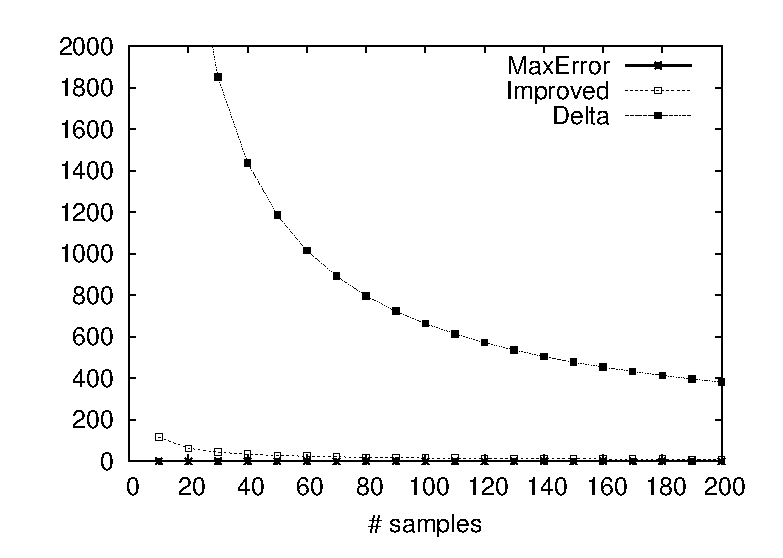
\includegraphics[width=.9\textwidth]{cos_normal_apprx_error.eps}
\caption{\textsf{MaxError}s and upper bounds for cosine similarity with normal distribution.}
\label{fig:cnae}
\end{minipage}
\hspace{1cm}
\begin{minipage}{.45\textwidth}
\centering
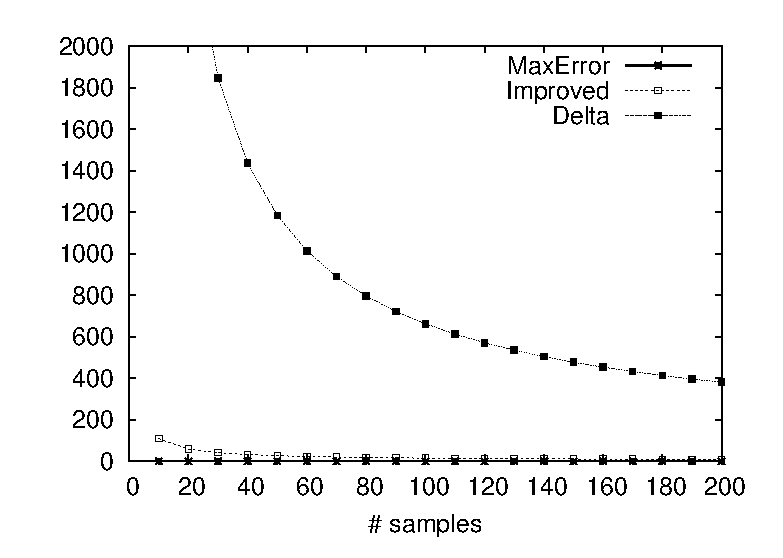
\includegraphics[width=.9\textwidth]{cos_uniform_apprx_error.eps}
\caption{\textsf{MaxError} and upper bounds for cosine similarity with uniform distribution.}
\label{fig:cuae}
\end{minipage}
\end{figure}

Figure \ref{fig:cnae} and Figure \ref{fig:cuae} present the maximum approximation errors and upper bound given by Algorithm \ref{alg:csa} for the synthesized data sets.
Here \textsf{MaxError} denotes the maximum absolute error among all the vector pairs, i.e.,
$$\textsf{MaxError} = \max_{u,v\in V,u\not= v} |\widetilde{Sim}(u,v) - Sim(u,v)|,$$
where $\widetilde{Sim}(u,v)$ is the approximated similarity between $u$ and $v$ given by our algorithms. The upper bound \textsf{Delta} is the $\Delta$ given in Algorithm \ref{alg:csa}, and we use the improved bound given in Section \ref{sec:imprb}. For the improved bound, we observe that with overwhelming probability, each feature product between any two vectors is less than 20.0 when $m=1000$. Hence we choose the adjusted parameter $\hat{m} = 20.0$. See Section \ref{sec:imprb} for details. 
For both figures, when more samples are drawn, the maximum absolute errors and upper bounds decrease. Also our improved upper bounds are significantly tighter than the bounds by $m$, but they are still much larger than the maximum absolute errors. Hence our theoretical bounds are still quite loose. However, our improved bounds can be sufficient for practical use. For uniform distribution, by 200 samplings, we can guarantee that the maximum absolute error among all the vector pairs is less than 0.005 with probability at least 99.99\%. Note that we have normalized the cosine similarities to be between 0 and 1. Similarly for normal distribution, by 200 samplings we can guarantee that with probability at least 99.99\%, the maximum absolute error is less than 0.005. However, the actual maximum error is only 0.001. Thus our bound is still quiteite loose.

\begin{figure}[!t]
\centering
\begin{minipage}{.45\textwidth}
\centering
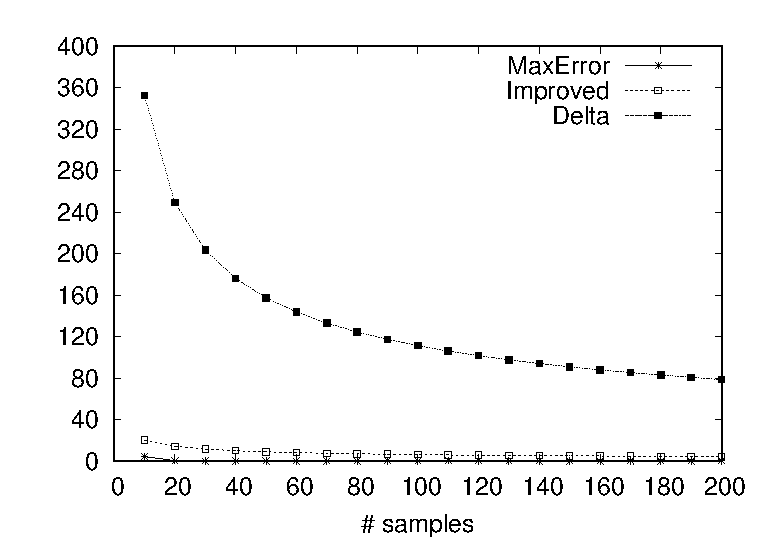
\includegraphics[width=.9\textwidth]{cos_arxiv_apprx_error.eps}
\caption{\textsf{MaxError}s and upper bounds for cosine similarity for \texttt{Cit-HepPh}.}
\label{fig:arxiv}
\end{minipage}
\hspace{1cm}
\begin{minipage}{.45\textwidth}
\centering
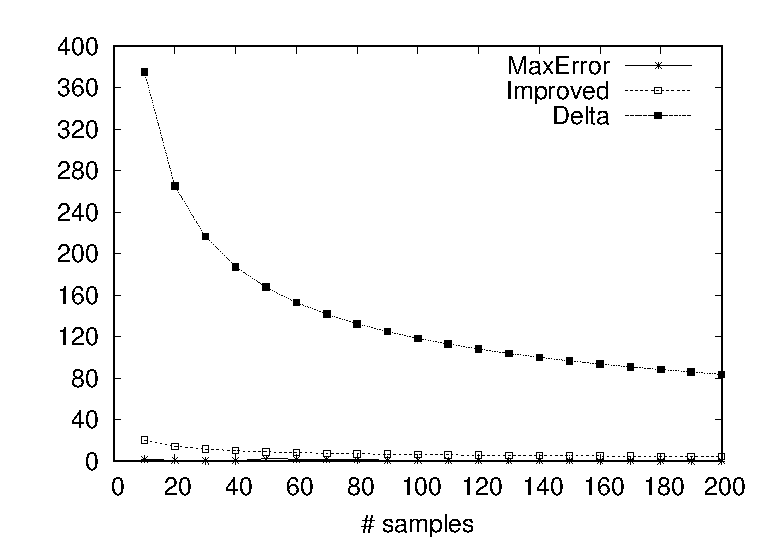
\includegraphics[width=.9\textwidth]{cos_email_apprx_error.eps}
\caption{\textsf{MaxError} and upper bounds for cosine similarity for \texttt{Email-Enron}.}
\label{fig:email}
\end{minipage}
\end{figure}

Figure \ref{fig:arxiv} and Figure \ref{fig:email} give the maximum approximation errors and upper bound given by Algorithm \ref{alg:csa} for the real-world data sets. Since there are more features (more than 30K), the upper bounds cannot be as tight as before. However, for \texttt{Cit-HepPh}, only 200 samples can guarantee an upper bound 0.015, which is quite small compared to the number of features. 

\begin{figure}[!t]
\centering
\begin{minipage}{.45\textwidth}
\centering
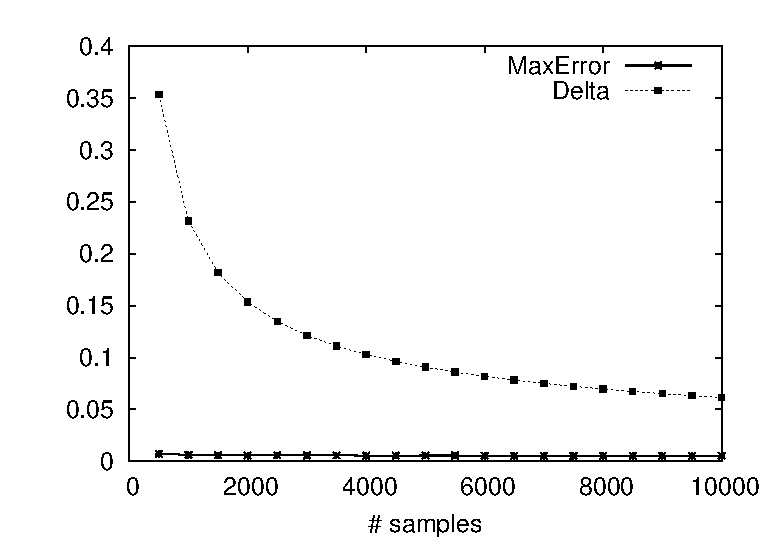
\includegraphics[width=.9\textwidth]{simrank_rg_apprx_error.eps}
\caption{\textsf{MaxError} and upper bounds for SimRank with random graph model.}
\label{fig:rgae}
\end{minipage}
\hspace{1cm}
\begin{minipage}{.45\textwidth}
\centering
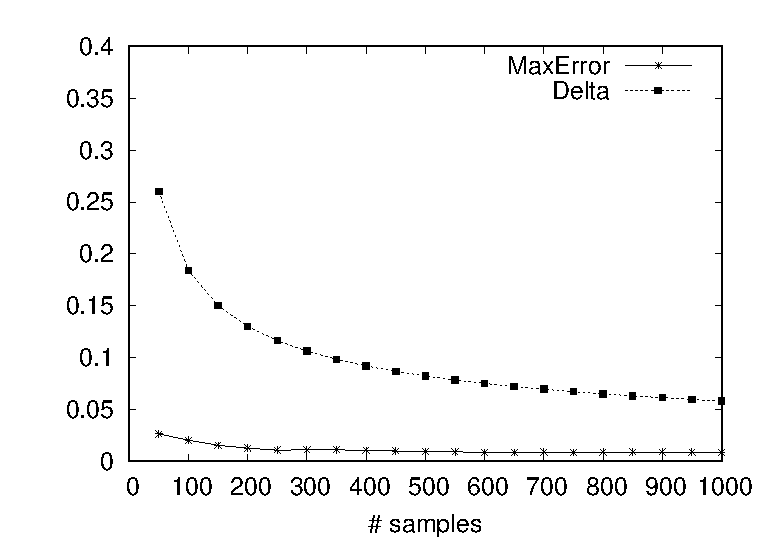
\includegraphics[width=.9\textwidth]{simrank_sw_apprx_error.eps}
\caption{\textsf{MaxError} and upper bounds for SimRank with small-world model.}
\label{fig:swae}
\end{minipage}
\end{figure}

Figure \ref{fig:rgae} and Figure \ref{fig:swae} present the approximation errors and upper bound given by Algorithm \ref{alg:sra} for the synthesized data sets.
Here the upper bound \textsf{Delta} is given in Algorithm \ref{alg:sra}. \textsf{MaxError} is same as before. 
For both figures, when more samples are drawn, the maximum absolute errors and upper bounds decrease. Note that even though our bounds are still quite loose compared to the maximum absolute errors, they can be practically used. For random graph model, by taking 1000 samples, we can guarantee that the maximum absolute error among all the node pairs is less than 0.059 with probability at least 99.99\%, and the maximum error is only 0.0057. For small-world model, by taking 1000 samples, we can guarantee that the maximum absolute error is less than 0.058 with probability at least 99.99\%. Note that the actual maximum error is about 0.009, which is still much smaller than our bounds.

\begin{figure}[!t]
\centering
\begin{minipage}{.45\textwidth}
\centering
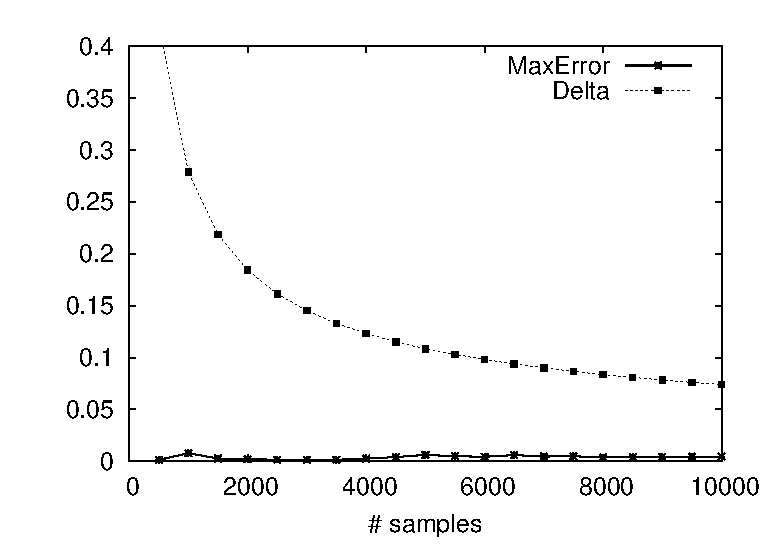
\includegraphics[width=.9\textwidth]{simrank_twitter_apprx_error.eps}
\caption{\textsf{MaxError} and upper bounds for SimRank for the network from \texttt{ego-Twitter}.}
\label{fig:twitter}
\end{minipage}
\hspace{1cm}
\begin{minipage}{.45\textwidth}
\centering
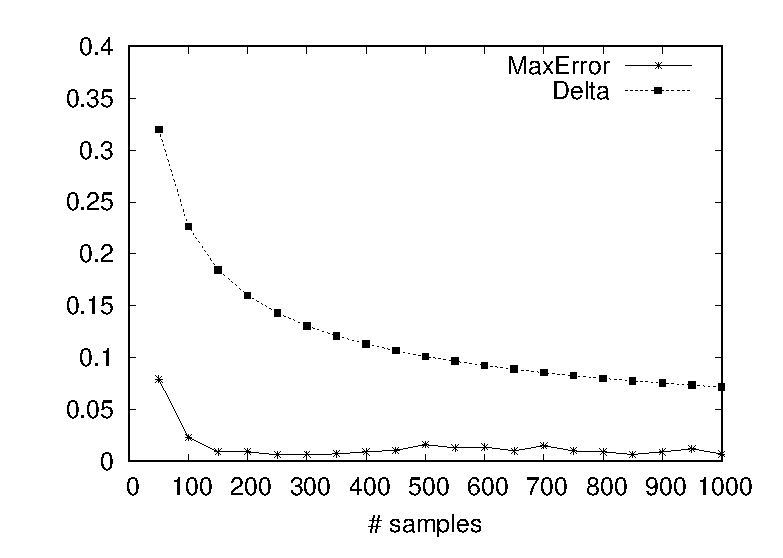
\includegraphics[width=.9\textwidth]{simrank_gplus_apprx_error.eps}
\caption{\textsf{MaxError} and upper bounds for SimRank for the network from \texttt{ego-Gplus}.}
\label{fig:gplus}
\end{minipage}
\end{figure}

Figure \ref{fig:twitter} and Figure \ref{fig:gplus} give the maximum approximation errors and upper bound given by Algorithm \ref{alg:sra} for the real-world data sets. The upper bounds are not as tight as before. For \texttt{ego-Twitter}, 1000 samples can guarantee an upper bound of 0.067, while the acutal maximum error is 0.02. For \texttt{ego-Gplus}, 1000 samples can guarantee an upper bound of 0.072, which is almost time times the actual maximum error.

\subsection{Running Time}
\begin{figure}[!t]
\centering
\begin{minipage}{.45\textwidth}
\centering
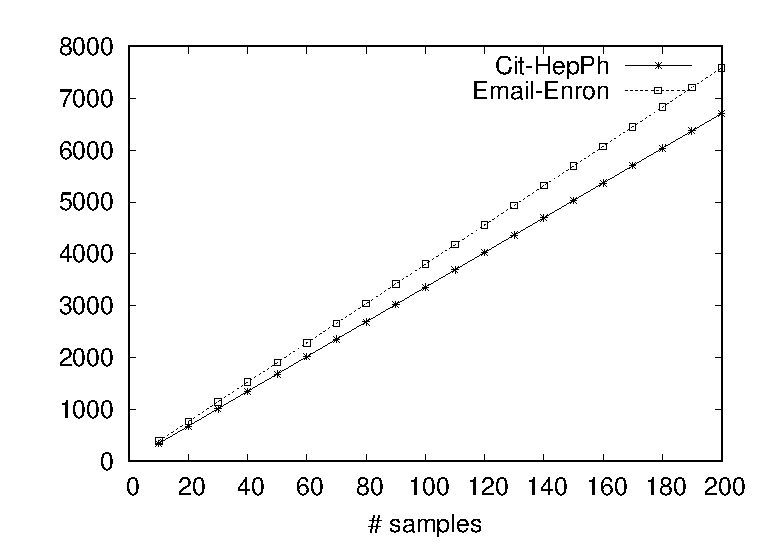
\includegraphics[width=.9\textwidth]{cos_runtime.eps}
\caption{Running time (ms) of Algorithm \ref{alg:csa} given sample sizes.}
\label{fig:run_cos}
\end{minipage}
\hspace{1cm}
\begin{minipage}{.45\textwidth}
\centering
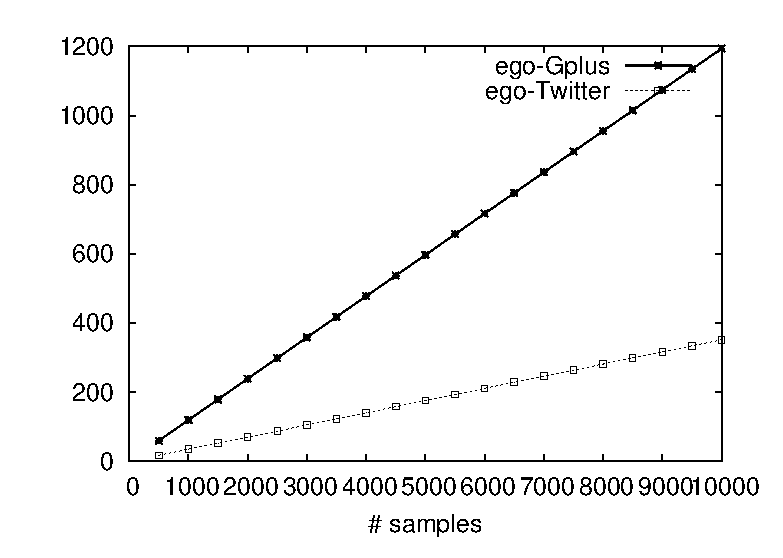
\includegraphics[width=.9\textwidth]{simrank_runtime.eps}
\caption{Running time (ms) of Algorithm \ref{alg:sra} given sample sizes.}
\label{fig:run_sr}
\end{minipage}
\end{figure}

Figure \ref{fig:run_cos} and Figure \ref{fig:run_sr} give the running time of our algorithms on the real-world data sets given the sample sizes. Here we did not use any parallelism or detection techniques to implement our algorithms. Note that in APSS we need to compute for each pair of objects. The number of such pairs grows quadratically. As a result when the sample size is large, the computation can take a few hours. A good news is that since the computation of each pair is independent from each other, the approximation algorithms can be easily distributed over multiple cores.

\section{Conclusion and Future Research}
\label{sec:con}
In this paper we have given two approximation algorithms (on cosine similarity and SimRank respectively) for all-pairs similarity search. 
A rigorous analysis using Rademacher average has been presented. 
{\color{black}As an important application, we have discussed how to use our approximations to efficiently tune the parameters and improve the performance of the popular LSH-based dissimilarity detection. }
We also have evaluated their performance by experiments on both synthesized and real-world data sets. The results show that our algorithms can precisely approximate the similarities with acceptable time complexity and error probability. 

We note that the upper bounds in this paper still have some space to improve. In the experiments our upper bounds are roughly 5 to 10 times the maximum absolute errors. In the proofs it is unclear whether the bounds we have used are the best possible. Hence the algorithms could be improved. Also it can be an interesting topic how to more efficiently use parallelism in APSS samplings.

%\bibliographystyle{./IEEEtran}
\bibliographystyle{plain}
\bibliography{./cos}

\section{Appendix}
\subsection{Proof of Theorem \ref{thm:finite}}
First, for any $\epsilon > 0$,
$$\begin{aligned}
\Pr[U_S(F) > \epsilon] =& \Pr[\exists f\in F, A_S(f) - A_D(f) > \epsilon] \\
\leq & \sum_{f\in F} \Pr[A_S(f) - A_D(f) > \epsilon] \\
=& \sum_{f\in F} \Pr[\frac{1}{k} \sum_{i=1}^k f(s_i) - A_D(f) > \epsilon]. \\
\end{aligned}$$ 
By Hoeffding's inequality \cite{BBL04} we have
$$\Pr[\frac{1}{k} \sum_{i=1}^k f(s_i) - A_D(f) > \epsilon] \leq \exp\left(-\frac{2k\epsilon^2}{m^2}\right).$$
Hence
$$\Pr[U_S(F) > \epsilon] \leq |F| \exp\left(-\frac{2k\epsilon^2}{m^2}\right).$$
Similarly one can show that
$$\Pr[\sup_{f\in F} [ A_D(f) - A_S(f) ] > \epsilon] \leq |F| \exp\left(-\frac{2k\epsilon^2}{m^2}\right).$$
Thus putting the two cases together,
$$\Pr[\sup_{f\in F} | A_S(f) - A_D(f) | > \epsilon] \leq 2|F| \exp\left(-\frac{2k\epsilon^2}{m^2}\right).$$
Equivalently for any $\delta>0$, with probability at least $1-\delta$,
$$\sup_{f\in F} | A_S(f) - A_D(f) | \leq m\sqrt{\frac{\log(2|F|) + \log(1/\delta)}{2k}}.$$
We have obtained the desired upper bound in Theorem \ref{thm:finite}.

\subsection{Proof of Theorem \ref{thm:main}}
In this section, we show our main result (Theorem \ref{thm:main}).
We start from the definition of self bounding function \cite{Oneto13}.
\begin{definition}
Let $s_1$, $s_2$, $\cdots$, $s_k$ be independent random variables taking values from a set $D$. A function $f: D^k \to [0, +\infty]$ is a self bounding function if there exists a constant $c$ and a function $g: D^{k-1}\to \mathbb{R}$ such that for any $s_1$, $\cdots$, $s_{j-1}$, $s_{j+1}$, $\cdots$, $s_k \in D$, the following conditions hold:
$$0 \leq f(s_1, \cdots, s_k) - g(s_1,\cdots, s_{j-1}, s_{j+1}, \cdots, s_k) \leq c,$$
$$\sum_{j=1}^k [f(s_1, \cdots, s_k) - g(s_1,\cdots, s_{j-1}, s_{j+1}, \cdots, s_k)] \leq f(s_1, \cdots, s_k).$$
\end{definition}

The following concentration inequality can be achieved for self bounding functions \cite{BLM99}.

\begin{lemma}
\cite{BLM99} If a function $Z = f(s_1,\cdots,s_k)$ is a self bounding function with constant $c$, then for $t \leq \E Z$,
$$\Pr[\E Z - Z \geq t] \leq \exp\left(-\frac{t^2}{2c\E Z}\right).$$
For $t > \E Z$, the left probability is zero trivially.
Here we take randomness over $s_1$, $s_2$, $\cdots$, $s_k$.
\end{lemma}

By using the above lemma, we can show a similar inequality for Rademacher average. 

\begin{lemma}
\label{lem1}
$$\Pr[\E R_S(F) \geq R_S(F) + t] \leq \exp\left(-\frac{kt^2}{4m\E R_S(F)}\right),$$
where $\E$ takes randomness over the samplings $s_1$, $s_2$, $\cdots$, $s_k$.
\end{lemma}
\begin{proof}
It suffices to show that $R_S(F)$ is a self bounding function with constant $c=2m/k$.
Define
$$Z = R_S(F) = \E_\sigma \sup_{f\in F} \left[\frac{2}{k}\sum_{i=1}^k \sigma_i f(s_i) \right],$$
$$G_j = \E_\sigma \sup_{f\in F} \left[\frac{2}{k}\sum_{i\not= j} \sigma_i f(s_i) \right].$$
It is clear that $Z$ is non-negative:
$$Z \geq \sup_{f\in F} \left[ \E_\sigma \frac{2}{k}\sum_{i=1}^k \sigma_i f(s_i) \right]=0.$$
Also it is clear that $Z \geq G_j$ for each $j$: suppose $\tilde{f}$ achieves the supreme of $G_j$. Then
$$\begin{aligned}
G_j &= \E_\sigma \left[\frac{2}{k}\sum_{i=1}^k \sigma_i \tilde{f}(s_i) - \frac{2}{k} \sigma_j \tilde{f}(s_j)\right] \\
&= \E_\sigma \left[\frac{2}{k}\sum_{i=1}^k \sigma_i \tilde{f}(s_i)\right] - \E_\sigma \left[ \frac{2}{k} \sigma_j \tilde{f}(s_j)\right] \\
&= \E_\sigma \left[\frac{2}{k}\sum_{i=1}^k \sigma_i \tilde{f}(s_i) \right]  \leq Z.
\end{aligned}$$
Next we show $Z- G_j \leq 2m/k =c$:
$$\begin{aligned}
G_j &= \E_\sigma \sup_{f\in F} \left[ \frac{2}{k} \sum_{i=1}^k \sigma_i f(s_i) - \frac{2}{k} \sigma_j f(s_j) \right] \\
&\geq \E_\sigma \sup_{f\in F} \left[ \frac{2}{k} \sum_{i=1}^k \sigma_i f(s_i) \right] - \E_\sigma \sup_{f\in F} \left[ \frac{2}{k} \sigma_j f(s_j) \right] \\
&\geq \E_\sigma \sup_{f\in F} \left[ \frac{2}{k} \sum_{i=1}^k \sigma_i f(s_i) \right] - \frac{2m}{k}.
\end{aligned}$$
Finally we need to verify $\sum_{j=1}^k Z-G_j \leq Z$:
$$\begin{aligned}
\sum_{j=1}^k G_j &= \E_\sigma \sum_{j=1}^k \sup_{f\in F} \left[ \frac{2}{k}\sum_{i\not= j} \sigma_i f(s_i) \right]\\
&\geq \E_\sigma \sup_{f\in F}\left[ \frac{2}{k} \sum_{j=1}^k \sum_{i\not= j} \sigma_i f(s_i) \right]\\
&=\frac{2(k-1)}{k} \E_\sigma \sup_{f\in F}\left[\sum_{j=1}^k \sigma_i f(s_i) \right] = (k-1)Z.
\end{aligned}$$
\end{proof}

We still need the following lemma on the relation between uniform deviation and Rademacher average.

\begin{lemma}
\label{lem2}
$$\E \sup_{f\in F} [ A_S(f) - A_D(f) ] \leq \E R_S(F),$$
$$\E \sup_{f\in F} [ A_D(f) - A_F(f) ] \leq \E R_S(F).$$
Here we take randomness over the $k$ samplings.
\end{lemma}
\begin{proof}
The proof idea is based on ghost samplings, i.e., independently draw another $k$ samples: $s_1'$, $\cdots$, $s_k'$, and then we have
$$A_D(f) = \frac{1}{m}\sum_{i=1}^m f(i) = \E \frac{1}{k} \sum_{j=1}^k f(s_j'),$$
where $\E$ takes randomness over the $k$ ghost samples.
Thus
$$\begin{aligned}
\E \sup_{f\in F} [ A_S(f) - A_D(f) ] &= \E \sup_{f\in F} \left[\frac{1}{k} \sum_{i=1}^k f(s_i) - \E \frac{1}{k} \sum_{j=1}^k f(s_j') \right]\\
&\leq \E \sup_{f\in F} \left[\frac{1}{k} \sum_{i=1}^k f(s_i) - \frac{1}{k} \sum_{j=1}^k f(s_j') \right].\\
\end{aligned}$$
Since all the samples $s$, $s'$ are independently identically distributed, flipping the sign of $f(s_i) - f(s_i')$ will not change the expected supreme, i.e.,
$$\E \sup_{f\in F} \left[\frac{1}{k} \sum_{i=1}^k f(s_i) - \frac{1}{k} \sum_{j=1}^k f(s_j') \right] = \E \sup_{f\in F} \frac{1}{k} \sum_{i=1}^k \left[\sigma_i (f(s_i) - f(s_i')) \right],$$
where $\sigma_i$ is uniformly distributed over $\{-1, 1\}$.
Since 
$$\E \sup_{f\in F} \frac{1}{k} \sum_{i=1}^k \left[\sigma_i (f(s_i) - f(s_i')) \right] \leq 2 \E \sup_{f\in F} \frac{1}{k} \sum_{i=1}^k \sigma_i f(s_i)  = \E R_S(F),$$
we have shown the first inequality. The second inequality is analogous.
\end{proof}

We also need McDiarmid's inequality \cite{M89}.
\begin{lemma}
\cite{M89} Let $s_1$, $\cdots$, $s_k$ be independent random variables taking values from a set $D$. Suppose a function $h: D^k \to \mathbb{R}$ satisfies
$$\sup_{x_1,\cdots,x_k,x_i'\in D} |h(x_1,\cdots,x_k) - h(x_1,\cdots,x_{i-1},x_i',x_{i+1},\cdots,x_k)| \leq c_i$$
for some constants $c_i$ and every $1\leq i \leq k$. Then for any $t>0$, we have
$$\Pr[h(s_1,\cdots,s_k) - \E h(s_1,\cdots,s_k) \geq t] \leq \exp\left(-\frac{2t^2}{\sum_{i=1}^k c_i^2}\right).$$
\end{lemma}

By the above three lemmas, we can bound the difference between true average and sampled average as follows.
\begin{lemma}
$$\begin{aligned}
&\Pr\left[\sup_{f\in F} |A_D(f) - A_S(f)| \geq R_S(F) + t\right] \\
\leq& 4\exp\left(-\frac{2kt^2}{(m+\sqrt{8m\E R_S(F)})^2} \right).\end{aligned}$$
\end{lemma}
\begin{proof}
First by Lemma \ref{lem2},
$$\begin{aligned}
&\Pr\left[\sup_{f\in F} [A_D(f) - A_S(f)] \geq R_S(F) + t\right] \\
\leq& \Pr\left[\sup_{f\in F} [A_D(f) - A_S(f)] \geq \E\sup_{f\in F} [A_D(f) - A_S(f)] + at\right] \\
&+ \Pr\left[\E R_S(F) \geq R_S(F)+(1-a)t\right] \\
\end{aligned}$$
for any $a\in [0,1]$. Let
$$h(s_1,\cdots,s_k) = A_D(f) - A_S(f) = A_D(f) - \frac{1}{k}\sum_{i=1}^k f(s_i).$$
It is clear that 
$$\begin{aligned}
&\sup_{x_1,\cdots,x_k,x_i'\in D} |h(x_1,\cdots,x_k) - h(x_1,\cdots,x_{i-1},x_i',x_{i+1},\cdots,x_k)| \\
=&\sup_{x_1,\cdots,x_k,x_i'\in D} \left|\frac{1}{k}\sum_{j=1, j\not=i}^k f(x_j)+\frac{1}{k}f(x_i') - \frac{1}{k}\sum_{i=1}^k f(x_i)\right| \\
=&\sup_{x_1,\cdots,x_k,x_i'\in D} \left|\frac{1}{k}f(x_i') - \frac{1}{k} f(x_i)\right| \leq \frac{m}{k}.
\end{aligned}$$
By McDiarmid's inequality,
$$\begin{aligned}
&\Pr\left[\sup_{f\in F} [A_D(f) - A_S(f)] \geq \E\sup_{f\in F} [A_D(f) - A_S(f)] + at\right] \\
\leq& \exp\left(-\frac{2a^2t^2}{\sum_{i=1}^k m^2/k^2}\right)
=\exp\left(-\frac{2ka^2t^2}{m^2}\right).
\end{aligned}$$

By Lemma \ref{lem1},
$$\Pr\left[\E R_S(F) \geq R_S(F)+(1-a)t\right] \leq \exp\left(-\frac{k(1-a)^2t^2}{4m\E R_S(F)}\right).$$
Let $a = 1/(1+\sqrt{8\E R_S(F) / m})$. Then putting everything together, we have 
$$\begin{aligned}
&\Pr\left[\sup_{f\in F} [A_D(f) - A_S(f)] \geq R_S(F) + t\right] \\
\leq& 2\exp\left(-\frac{2kt^2}{(m+\sqrt{8m\E R_S(F)})^2} \right).\end{aligned}$$
Similarly one can show 
$$\begin{aligned}
&\Pr\left[\sup_{f\in F} [A_S(f) - A_D(f)] \geq R_S(F) + t\right] \\
\leq& 2\exp\left(-\frac{2kt^2}{(m+\sqrt{8m\E R_S(F)})^2} \right).\end{aligned}$$
Thus we have the inequality as desired.
\end{proof}
By the above lemma we have the following important corollary.
\begin{corollary}
With probability at least $1-\delta$, we have
$$\sup_{f\in F}|A_S(f) - A_D(f)| \leq R_S(F) + (m+\sqrt{8m \E R_S(F)})\sqrt{\frac{\log \frac{4}{\delta}}{2k}}.$$
\end{corollary}

We still need to upper bound $\E R_S(F)$. By Lemma \ref{lem1}, with probability at least $1-\delta$,
$$\E R_S(F) \leq R_S(F) + \sqrt{4m\E R_S(F)\frac{\log \frac{1}{\delta}}{k}}.$$
Or equivalently,
$$\sqrt{\E R_S(F)} \leq \sqrt{\frac{m}{k}\log \frac{1}{\delta}} + \sqrt{\frac{m}{k}\log \frac{1}{\delta} + R_S(F)}.$$
Hence with probability at least $1-2\delta$, we have
$$\sup_{f\in F}|A_S(f) - A_D(f)| \leq R_S(F) + \left(m+m\sqrt{\frac{8}{k}\log \frac{1}{\delta}} + m\sqrt{\frac{8}{k}\log \frac{1}{\delta} + \frac{8R_S(F)}{m}}\right)\sqrt{\frac{\log \frac{4}{\delta}}{2k}}.$$
We have shown Theorem \ref{thm:main}.


\subsection{Proof of Theorem \ref{thm2}}
For any $s>0$, by Jensen's inequality,
$$\begin{aligned}
\exp(skR_S(F)) & = \exp\left(2s\E_\sigma \sup_{f\in F} \sum_{i=1}^k \sigma_i f(s_i)\right) \\
&\leq \E_\sigma \exp\left(2s \sup_{f\in F} \sum_{i=1}^k \sigma_i f(s_i)\right) \\
&\leq \E_\sigma \sum_{f\in F} \exp\left(2s\sum_{i=1}^k \sigma_i f(s_i)\right).
\end{aligned}$$
By Hoeffding's Lemma \cite{H63},
$$\begin{aligned}
&\E_\sigma \sum_{f\in F} \exp\left(2s\sum_{i=1}^k \sigma_i f(s_i)\right) \\
\leq & \sum_{f\in F}\prod_{i=1}^k \exp\left(2s^2f(s_i)^2\right) \\
=& \sum_{f\in F} \exp\left(2s^2\sum_{i=1}^k f(s_i)^2\right).
\end{aligned}$$
Let $\ell^2 = \sup_{f\in F}\sum_{i=1}^k f(s_i)^2$, and then
$$\sum_{f\in F} \exp\left(2s^2\sum_{i=1}^k f(s_i)^2\right) \leq |F| \exp\left(2s^2\ell^2\right).$$
Thus
$$R_S(F) \leq \frac{1}{sk}(\log|F| + 2s^2\ell^2),$$
for any $s>0$. It turns out that to minimize the right hand side of the above equation, we have
$$s = \sqrt{\frac{\log|F|}{2\ell^2}}.$$
Then
$$R_S(F) \leq \frac{\ell}{k}\sqrt{8\log |F|}.$$ 


\subsection{Discussions of Theorem \ref{thm:new}}
Theorem \ref{thm:new} can be treated as a special case of Theorem \ref{thm:finite} and Theorem \ref{thm:main} when $m=c$. All the reasoning will not be affected and thus the desired bound follows.
\end{document}
